\section{Mathematische Grundlagen}

Die Berechnungen in dieser Arbeit finden alle im reellen Raum statt, also in den
Vektorräumen $\PimiddyReell^n$, wobei $n \in \{1,2,3\}$. Die Berechnungen werden meistenens
auf \PimiddyBegriff{Vektorfeldern} und \PimiddyBegriff{Skalarfeldern}
angewendet, daher sollen diese Begriffe und die zugehörigen Operationen hier
eingeführt werden. Des weiteren werden wir die Operationen
\emph{diskretisieren}, da wir numerische Lösungen verfolgen und keine
analytischen.

\subsection{Kontinuierlich}

Ein \PimiddyBegriff{Vektorfeld} $\vec{u}$ ist eine Abbildung

\begin{equation*}
\vec{u} \colon \PimiddyReell^n \to \PimiddyReell^n
\end{equation*}

die einem Punkt im Raum einen Pfeil zuordnet. So kann z.B. jedem Punkt im Raum
die Fließgeschwindigkeit des Fluids an diesem Punkt zugeordnet werden. Wir
definieren $\PimiddyVectorfields(\PimiddyReell^n)$ als die Menge aller
Vektorfelder.

Analog ist ein \PimiddyBegriff{Skalarfeld} $p$ eine Abbildung

\begin{equation*}
p \colon \PimiddyReell^n \to \PimiddyReell
\end{equation*}

welche einem Punkt im Raum einen skalaren Wert zuordnet. Beispielsweise könnte
für jeden Punkt im Raum die dortige Temperatur in einem Skalarfeld gespeichert
sein. Wir definieren $\PimiddyScalarfields(\PimiddyReell^n)$ als die Menge aller
Skalarfelder.

\begin{figure}
	\begin{subfigure}[b]{0.5\textwidth}
		\centering
		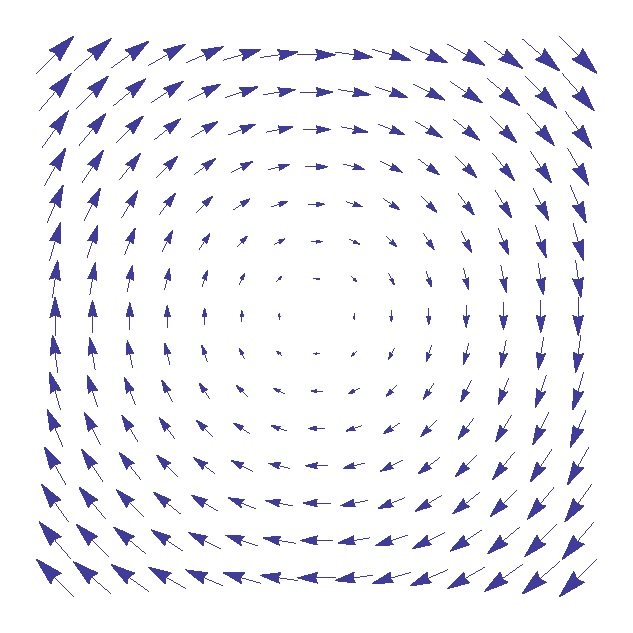
\includegraphics[width=\textwidth]{images/vectorfield}
		\caption{Ein Vektorfeld}
		\label{mathematics_vectorfield}
	\end{subfigure}
	~
	\begin{subfigure}[b]{0.5\textwidth}
		\centering
		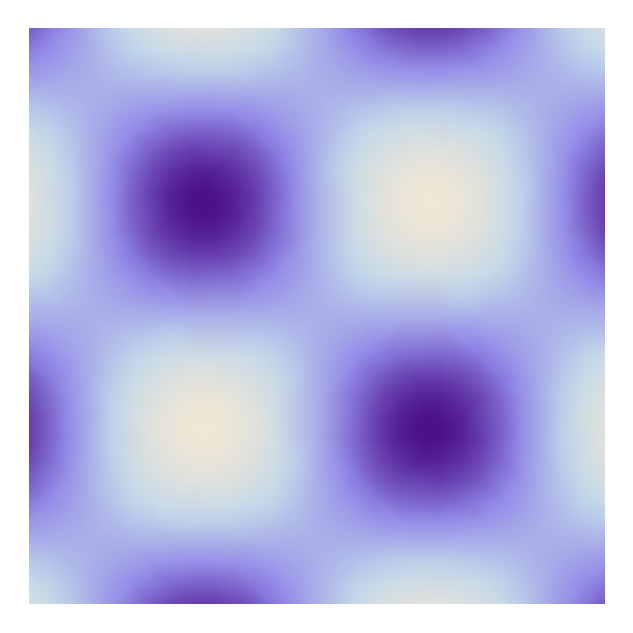
\includegraphics[width=\textwidth]{images/scalarfield}
		\caption{Ein Skalarfeld}
		\label{mathematics_scalarfield}
	\end{subfigure}
	\caption{Die betrachteten Feldtypen}
\end{figure}

Sei $p$ ein dreidimensionales Skalarfeld, dann ist der \PimiddyBegriff{Gradient}
$\PimiddyGrad p$ definiert als:

\begin{gather}
\PimiddyGrad \colon \PimiddyScalarfields \to \PimiddyVectorfields \\
\PimiddyGrad p
=
\left( \frac{\partial p}{\partial x},\frac{\partial p}{\partial y},\frac{\partial p}{\partial z} \right)
\end{gather}

Der Gradient eines Skalarfeldes ist also ein Vektorfeld, nämlich das Vektorfeld
der partiellen Ableitungen. Genauso wie die Ableitung eines Graphen die Steigung
an jedem Punkt angibt, so zeigt der Gradient eines Feldes in die Richtung des
steilsten Anstiegs. Seine Länge gibt die Größe Steigung an. Der Gradient des
negativen Skalarfeldes $-p$ zeigt folglich in Richtung des größten Gefälles.

Ist ein Vektorfeld $\vec{u}$ differenzierbar (was wir in dieser Arbeit für alle
Vektorfelder annehmen), dann ist die \PimiddyBegriff{Divergenz} auf dem
Feld definiert als

\begin{gather}
\PimiddyDiv \colon \PimiddyVectorfields \to \PimiddyScalarfields \\
\PimiddyDiv \vec{u}
=
\frac{\partial u_x}{\partial x} +
\frac{\partial u_y}{\partial y} +
\frac{\partial u_z}{\partial z}
\end{gather}

Hier sind $u_x,u_y,u_z$ die einzelnen Komponenten des Vektorfeldes. Die
Divergenz eines Vektorfelds ist also ein Skalarfeld. Dieses Skalarfeld kann
gedeutet werden als \PimiddyQuotes{Quellendichte} des ursprünglichen
Vektorfeldes. Ein Feld $\vec{u}$, was $\PimiddyDiv \vec{u}=0$ erfüllt, heißt folglich
\PimiddyBegriff{quellenfrei}.

Auf Vektorfeldern ist schließlich noch die \PimiddyBegriff{Rotation} definiert:

\begin{gather}
\PimiddyDiv \colon \PimiddyVectorfields \to \PimiddyVectorfields \\
\PimiddyDiv \vec{u}
=
\left(
	\begin{array}{c}
		\frac{\partial u_z}{\partial y} - \frac{\partial u_y}{\partial z} \\
		\frac{\partial u_x}{\partial z} - \frac{\partial u_z}{\partial x} \\
		\frac{\partial u_y}{\partial x} - \frac{\partial u_x}{\partial y}
	\end{array}
\right)
\end{gather}

Wie der Name schon andeutet gibt sie für jeden Punkt des ursprünglichen
Vektorfeldes an, wie stark und in welche Richtung es rotiert. Stellt
man sich ein Windrad im Vektorfeld vor gibt die Rotation an, wie stark und in
welche Richtung es sich drehen würde. Im Zweidimensionalen ist die Rotation auch
definiert, hier ist sie allerdings nur ein Skalar, die Rotationsachse ist immer
die imaginäre \PimiddyQuotes{$z$-Achse} (siehe ). Ein Feld $\vec{u}$, was $\PimiddyRot
\vec{u}=0$ erfüllt, heißt \PimiddyBegriff{rotationsfrei}.

\begin{figure}
	\begin{subfigure}[b]{0.5\textwidth}
		\centering
		\includegraphics[width=\textwidth]{images/vector_field_rotation_arrows}
		\label{mathematics_image_vectorfield_rotation_arrows}
	\end{subfigure}
	~
	\begin{subfigure}[b]{0.5\textwidth}
		\centering
		\includegraphics[width=\textwidth]{images/vector_field_rotation}
	\end{subfigure}
	\caption{Ein 2D-Strömungsfeld, das um ein Hindernis herumfließt mit dazugehöriger Rotation. Negative Rotation ist rot gekennzeichnet, positive in blau.}
\end{figure}

In der Physik findet man den Gradienten und die Divergenz meist unter dem Symbol
$\nabla$ vereint. Je nachdem, ob es auf ein Vektor- oder ein Skalarfeld
angewendet wird, wechselt es die Bedeutung.
%Diese Notation wird in der Arbeit bevorzugt, da man die Symbole $\PimiddyGrad$ bzw. $\PimiddyDiv$ in der Literatur zu Fluiddynamik kaum vorfindet.

Schaltet man $\PimiddyGrad$ und $\PimiddyDiv$ hintereinander, erhält man den
\PimiddyBegriff{Laplace-Operator}:

\begin{gather}
\PimiddyLaplace \colon \PimiddyScalarfields \to \PimiddyScalarfields \\
\PimiddyLaplace p = \PimiddyDiv \PimiddyGrad p
\end{gather}

Manchmal wird auch das Symbol $\nabla^2$ für den Laplace-Operator benutzt. Im Dreidimensionalen ergibt sich:

\begin{equation}
\PimiddyLaplace p =
\frac{\partial^2 p}{\partial^2 x} +
\frac{\partial^2 p}{\partial^2 y} +
\frac{\partial^2 p}{\partial^2 z}
\end{equation}

Intuitiv misst der Operator für jeden Punkt $\vec{x}$ die Abweichung von
$p(\vec{x})$ zu Punkten in seiner Umgebung. Die diskretisierte Variante dieses
Operators wird deswegen in der Bildverarbeitung zum Erkennen von Kanten in
Bildern verwendet (siehe \autoref{mathematics_image_laplacian}).

Der Operator lässt sich auf nahe liegende Weise auf Vektorfelder erweitern, in drei Dimensionen
ergibt sich:

\begin{equation}
\PimiddyLaplace \vec{u} =
\left(
	\begin{array}{c}
		\PimiddyLaplace u_x \\
		\PimiddyLaplace u_y \\
		\PimiddyLaplace u_z
	\end{array}
\right)
\end{equation}

\begin{figure}
	\begin{subfigure}[b]{0.5\textwidth}
		\centering
		\includegraphics[width=\textwidth]{images/schloss_grey}
		\caption{Originalbild}
	\end{subfigure}
	~
	\begin{subfigure}[b]{0.5\textwidth}
		\centering
		\includegraphics[width=\textwidth]{images/schloss_grey_laplace}
		\caption{Das Bild nach Anwendung des Laplace-Operators}
		\label{mathematics_image_laplacian}
	\end{subfigure}
\end{figure}

\subsection{Diskret}

\subsubsection{Gittertypen}

Die hier vorgestellten Lösungsalgorithmen benutzen nicht den rellen Raum
$\PimiddyReell^n$ sondern ein endliches Gitter, also eine Teilmenge von
$\PimiddyGanz^n$.

In der Literatur findet man zwei Typen von Gittern: \PimiddyBegriff{kollokierte}
(\PimiddyEnglisch{collocated}) und \PimiddyBegriff{gestaffelte}
(\PimiddyEnglisch{staggered}).

\subsubsection{Diskrete Operatoren}

Die eben vorgestellten mathematischen Definitionen gehen von unendlichen,
kontinuierlichen Raum $\PimiddyReell^n$ aus. Für die Berechnungen werden wir
aber ein endliches, diskretes Gitter verwenden, also eine Teilmenge von
$\PimiddyGanz^n$. Folglich müssen die Operatoren in eine diskrete Form gebracht
werden.

\PimiddyTodo{Hier noch auf die Diskretisierungen eingehen (hier vielleicht auch Gittertypen kurz anschneiden?)}
